%======================================================================
% NewsAnalyzer Ubi-Media 2027 Submission Template (LLNCS)
% Local LLM + SBERT/Cofacts real-time fake news detection
%======================================================================

\documentclass[twoside]{llncs}
\usepackage[utf8]{inputenc}
\usepackage[T1]{fontenc}
\usepackage{upquote}
\usepackage{listings}
\usepackage[english]{babel}
\usepackage{url}
\usepackage{xurl}
\usepackage[hidelinks]{hyperref}
\usepackage{graphicx}
\usepackage{amsmath,amssymb}
\usepackage{booktabs}
\usepackage[expansion=false]{microtype}
\usepackage{float}
\usepackage{cite}
\usepackage{tikz}
\usetikzlibrary{arrows.meta, positioning}
\setlength{\textfloatsep}{8pt plus 2pt minus 2pt}
\setlength{\floatsep}{6pt plus 2pt minus 2pt}
\setlength{\intextsep}{6pt plus 2pt minus 2pt}

%======================================================================
% TITLE / AUTHOR
%======================================================================
\title{NewsAnalyzer: Real-Time Fake News Detection on Social Media\texorpdfstring{\\ \vspace{0.5em}\large}{ - }via Local Large Language Models and Semantic Retrieval}
\titlerunning{NewsAnalyzer: Real-Time Fake News Detection on Social Media}
\authorrunning{T. Lin and H. Lin}

\author{Tsangyu Lin\inst{1} \and Hui Lin\inst{1}\thanks{Corresponding author.}}

\institute{
Department of Computer Science and Information Engineering, \\
Tamkang University, New Taipei City 25137, Taiwan \\
\email{jefflin.je598@gmail.com, 121678@mail.tku.edu.tw}}

\begin{document}

\maketitle

%======================================================================
% ABSTRACT
%======================================================================
\begin{abstract}
This paper presents NewsAnalyzer, a real-time fake news detection system deploying a local large language model directly on client hardware for multi-dimensional credibility analysis---including structured viewpoint synthesis, inquiry targets, and contextual credibility scoring---without third-party cloud APIs, latency overheads, or privacy exposure. Unlike standard cloud API deployments, our system enforces strict JSON output via Ollama's grammar-constrained decoding (\texttt{format:\allowbreak json}), eliminating reasoning artifacts (e.g., thought markers) that trigger \texttt{JSON\-Decode\-Error} exceptions. The system integrates Sentence-BERT (SBERT) semantic embeddings over a localized Traditional Chinese fact-checking corpus (Cofacts) for nearest-neighbor retrieval. The resulting multi-signal assessment is rendered directly in the social feed via a Chrome Extension, providing robust misinformation deterrence for the Traditional Chinese social media ecosystem.
\keywords{fake news detection, large language models, local deployment, Gemma, JSON structured output, semantic search, system robustness, Chrome extension, Taiwan news}
\end{abstract}

%======================================================================
% 1 INTRODUCTION
%======================================================================
\section{Introduction}

Fake news on social networking services (SNS) has spread rapidly, posing severe challenges to public discourse. In Taiwan, social media represents a primary news channel where deceptive rumors and politically motivated disinformation distort public understanding. Despite substantial research on fake news detection, most existing benchmarks and tools remain tailored to English corpora and rely primarily on centralized social-graph signals, which suffer from propagation delays and lack the real-time responsiveness required for client-side assistance.

Traditional machine learning methods relying on bag-of-words, TF-IDF, or static lexical dictionaries struggle to capture nuanced semantic contexts and modern linguistic manipulation. Moreover, generative AI has made synthesized fake news increasingly sophisticated. In response, we propose an AI-driven, client-assisted system to evaluate the reliability of news content in real time, focusing on Traditional Chinese text on social media.

While frontier cloud-hosted LLMs exhibit strong contextual reasoning, deploying commercial cloud APIs inside an interactive browser extension introduces three critical engineering bottlenecks:
(1)~\textbf{Latency Overhead}: Network round-trip delays make cloud APIs ill-suited for synchronous browser feed analysis, where interactive assistance requires sub-second initial responses;
(2)~\textbf{Data Privacy Risks}: Cloud pipelines transmit sensitive browsing telemetry, reading habits, and post content to third-party endpoints; and
(3)~\textbf{Reasoning Artifact Contamination}: Unconstrained models often emit conversational filler, thought markers (\texttt{<thought>}), or markdown code fences (\texttt{```json}), causing downstream JSON parsers to crash.

To overcome these limitations, modern local LLM inference engines (such as Ollama~\cite{ollama2024}) combined with quantized model weights (GGUF format) enable high-throughput on-device inference for 12-billion-parameter models on consumer-grade GPUs. Processing queries locally preserves privacy and guarantees predictable latency bounded solely by local compute.

The contributions of this paper are summarized as follows:
\begin{itemize}\setlength{\itemsep}{2pt}
  \item We design a local fact-checking architecture executing on-device, providing sub-second TTFT ($\sim$200\,ms) and full data sovereignty without third-party API dependencies.
  \item We eliminate reasoning artifact contamination by enforcing grammar-constrained decoding via Ollama's \texttt{format:json} interface, achieving a 100\% JSON parsing rate over 100 benchmark runs.
  \item We develop a multi-signal scoring engine coupling local Gemma-4-12B~\cite{gemma4model, gemma2024} reasoning with Sentence-BERT (SBERT)~\cite{reimers2019sbert} semantic retrieval over a localized Cofacts~\cite{cofacts2020} database, reinforced by domain reputation, sentiment polarity, and recency signals.
  \item We empirically validate the system on an NVIDIA GeForce RTX 2080 Ti (22\,GB VRAM) environment, presenting real API benchmarks of throughput (46.7\,tok/s), memory footprint (9.2\,GB VRAM), and full-corpus 5-fold cross-validation on 2,292 verified claims (95.3\% accuracy at $\theta_{\text{sim}} = 0.72$).
\end{itemize}

%======================================================================
% 2 RELATED WORKS
%======================================================================
\section{Related Works}

The rapid spread of false information on digital platforms poses significant risks to public trust and social stability~\cite{wang2017liar, Bianchi2024trustworthiness}, making automated credibility evaluation an active research domain~\cite{guo2022survey}.

\subsection{Fact-Checking Platforms and Browser Extensions}
Fact-checking initiatives worldwide develop collaborative verification workflows and crowdsourced assessments~\cite{guo2022survey, pennycook2019fighting, allen2021scaling}. Guo et al. systematized automated fact-checking into claim detection, evidence retrieval, and verdict prediction~\cite{guo2022survey}. In Taiwan, the Cofacts community operates an open, crowdsourced rumor verification database~\cite{cofacts2020, lim2023factchecking}, cross-referenced with certified signatories of the International Fact-Checking Network (IFCN)~\cite{ifcn2020}, such as the Taiwan FactCheck Center (TFC)~\cite{tfc2023} and MyGoPen. To assist users during active web navigation, tools such as NewsGuard assess the editorial integrity of media outlets and display trust ratings alongside social feeds~\cite{Bianchi2024trustworthiness}. However, existing extensions predominantly evaluate static publisher reputations rather than analyzing the specific claims within an individual post. NewsAnalyzer differs by evaluating immediate post text through dynamic local LLM reasoning and real-time semantic evidence matching.

\subsection{Content-Based Detection and Dense Semantic Retrieval}
Content-based deception detection originally focused on stylometric features, syntax, and sentiment distributions~\cite{perez2018automatic, rashkin2017truth, potthast2018stylometric}. Wang established the LIAR benchmark to evaluate deep learning classifiers on structured political statements~\cite{wang2017liar}, while Transformer-based architectures such as BERT~\cite{devlin2019bert} improved contextual modeling across multilingual texts. Dense vector representations allow semantic similarity matching beyond surface keyword overlap. Sentence-BERT (SBERT) employs siamese networks to derive semantically meaningful sentence embeddings compared via cosine similarity~\cite{reimers2019sbert}. We utilize a multilingual SBERT model (\texttt{paraphrase-multilingual-MiniLM-L12-v2}) to embed incoming news text into a 384-dimensional latent space against pre-indexed fact-checked claims.

\subsection{Local LLM Inference and Comparative Positioning}
Quantization formats such as GGUF~\cite{gguf2023} and runtimes like Ollama~\cite{ollama2024} enable 12B-parameter models to operate efficiently on modern consumer-grade GPUs (7.5--9.2\,GB VRAM in Q4\_K\_M). The recent emergence of LLM-based credibility systems highlights different architectural trade-offs. \textbf{FreshLLMs}~\cite{vu2024freshllms} augments an LLM with live search-engine retrieval, but its pipeline is latency-bound by API round-trips and depends on third parties. \textbf{FacTool}~\cite{chern2023factool} offers a multi-domain factuality-detection framework as a post-hoc batch evaluator rather than a real-time interactive overlay. \textbf{ClaimBuster}~\cite{hassan2017claimbuster} detects check-worthy claims in political discourse without producing end-user verdicts. \textbf{dEFEND}~\cite{shu2019defend} demonstrates explainable fake news detection by coupling content with comments, but requires supervised training and is restricted to English. NewsAnalyzer differs in three concrete respects: (i)~it targets the Traditional Chinese misinformation ecosystem (Cofacts / TFC / MyGoPen); (ii)~it runs entirely on-device, eliminating network round-trips and privacy exposure; and (iii)~it produces an explainable JSON verdict in a single inference round via grammar-constrained decoding.

%======================================================================
% 3 METHODOLOGY
%======================================================================
\section{Methodology}

NewsAnalyzer comprises three integrated tiers: a client-side Chrome Extension for DOM extraction and overlay rendering, a lightweight local Flask backend acting as an inference router, and a dual-engine evaluation core combining Ollama-served Gemma-4-12B with an SBERT-based Cofacts retrieval engine.

\subsection{System Architecture}

\begin{figure}[!htbp]
\centering
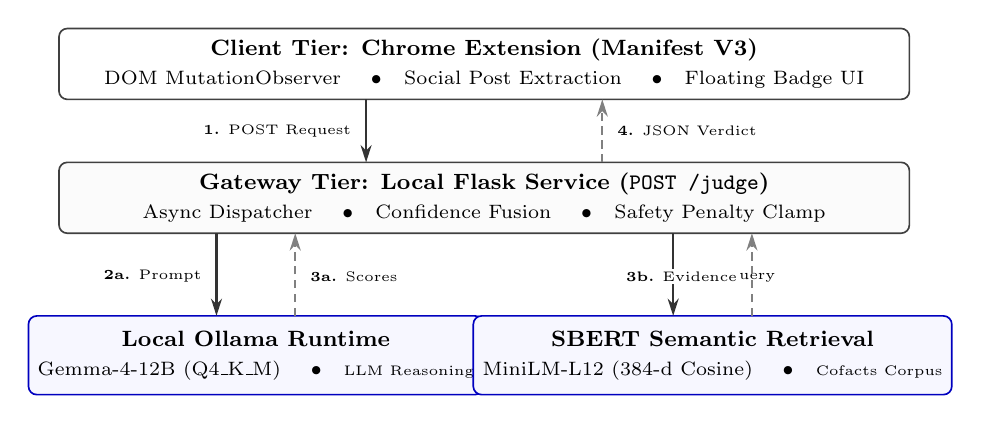
\begin{tikzpicture}[
  box/.style={draw=black!75, rounded corners=3pt, fill=white, align=center,
              font=\footnotesize, line width=0.6pt},
  srv/.style={draw=black!75, rounded corners=3pt, fill=gray!3, align=center,
              font=\footnotesize, line width=0.6pt},
  eng/.style={draw=blue!75!black, rounded corners=3pt, fill=blue!3, align=center,
              font=\footnotesize, line width=0.6pt},
  arr/.style={-{Stealth[length=2.2mm, width=1.4mm]}, thick, draw=black!80},
  revarr/.style={-{Stealth[length=2.2mm, width=1.4mm]}, thick, draw=black!50,
                 densely dashed},
  lbl/.style={font=\tiny, fill=white, inner sep=1pt}
]

  % ========== TIER 1: Client ==========
  \node[box, minimum width=10.8cm, minimum height=0.9cm] (t1) at (0, 3.3) {
    \textbf{Client Tier: Chrome Extension (Manifest V3)}\\[1pt]
    \scriptsize DOM MutationObserver \quad$\bullet$\quad
    Social Post Extraction \quad$\bullet$\quad
    Floating Badge UI
  };

  % ========== TIER 2: Gateway ==========
  \node[srv, minimum width=10.8cm, minimum height=0.9cm] (t2) at (0, 1.6) {
    \textbf{Gateway Tier: Local Flask Service (\texttt{POST /judge})}\\[1pt]
    \scriptsize Async Dispatcher \quad$\bullet$\quad
    Confidence Fusion \quad$\bullet$\quad
    Safety Penalty Clamp
  };

  % ========== TIER 3: Dual Cores ==========
  \node[eng, minimum width=4.8cm, minimum height=1.0cm] (ollama) at (-2.9, -0.4) {
    \textbf{Local Ollama Runtime}\\[1pt]
    \scriptsize Gemma-4-12B (Q4\_K\_M) \quad$\bullet$\quad \tiny LLM Reasoning
  };

  \node[eng, minimum width=4.8cm, minimum height=1.0cm] (sbert) at (2.9, -0.4) {
    \textbf{SBERT Semantic Retrieval}\\[1pt]
    \scriptsize MiniLM-L12 (384-d Cosine) \quad$\bullet$\quad \tiny Cofacts Corpus
  };

  % ======== ARROWS: T1 <-> T2 ========
  \draw[arr] (-1.5, 2.85) -- (-1.5, 2.05);
  \node[lbl, anchor=east] at (-1.65, 2.45)
    {\textbf{1.} POST Request};

  \draw[revarr] (1.5, 2.05) -- (1.5, 2.85);
  \node[lbl, anchor=west] at (1.65, 2.45)
    {\textbf{4.} JSON Verdict};

  % ======== ARROWS: T2 <-> Ollama ========
  \draw[arr] (-3.4, 1.15) -- (-3.4, 0.1);
  \node[lbl, anchor=east] at (-3.55, 0.6)
    {\textbf{2a.} Prompt};

  \draw[revarr] (-2.4, 0.1) -- (-2.4, 1.15);
  \node[lbl, anchor=west] at (-2.25, 0.6)
    {\textbf{3a.} Scores};

  % ======== ARROWS: T2 <-> SBERT ========
  \draw[arr] (2.4, 1.15) -- (2.4, 0.1);
  \node[lbl, anchor=west] at (2.55, 0.6)
    {\textbf{2b.} Query};

  \draw[revarr] (3.4, 0.1) -- (3.4, 1.15);
  \node[lbl, anchor=east] at (3.25, 0.6)
    {\textbf{3b.} Evidence};

\end{tikzpicture}
\caption{Layered architecture of NewsAnalyzer: the client extension communicates with the local Flask gateway, which dispatches requests to Ollama LLM and SBERT retrieval in parallel. Solid arrows denote requests; dashed arrows denote responses.}
\label{fig:arch}
\end{figure}

Figure~\ref{fig:arch} depicts the operational dataflow. When the user interacts with an analyzed post on social media, the Chrome extension extracts the article text, URL, and metadata from the document object model (DOM) and transmits a structured payload to the local server via \texttt{POST /judge}.

\subsubsection{Client-Side DOM Parsing (Manifest V3)}
The front end conforms to Google Chrome Manifest V3 specifications~\cite{chrome_mv3}. A content script attaches a \texttt{Mutation\allowbreak Observer} to the Facebook feed container. Whenever new post nodes are dynamically injected during user scrolling, the script inserts a lightweight assessment button. The extension restricts its network communications strictly to the local host address, preventing data egress.

\subsection{LLM-Driven Contextual Analysis}
Contextual analysis is performed by a quantized Gemma-4-12B model~\cite{gemma2024, gemma4model} hosted via Ollama. The zero-shot prompt enforces objective fact-checking guidelines tailored to Traditional Chinese social media. Rather than returning free-form text, the model is constrained via Ollama's formal JSON schema generator to output a single JSON object with four fields: \texttt{key\_points} (factual claims), \texttt{viewpoints} (contextual arguments, $<80$ chars), \texttt{credibility\_score} (integer in $[0, 100]$), and \texttt{analysis} (concise synthesis, $<100$ chars). Hyperparameters are configured with $\text{temperature} = 0.2$, $\text{num\_predict} = 400$, and $\text{think} = \texttt{false}$ for deterministic output. In production (\texttt{POST /judge}), the server invokes an ensemble routine (\texttt{deep\_analyze\_ensemble}), dispatching up to three concurrent requests and averaging returned scores.

\subsubsection{Prompt Template}
The LLM is invoked with a fixed zero-shot system prompt that combines the JSON schema with explicit Traditional-Chinese fact-checking instructions:

\begin{lstlisting}[basicstyle=\ttfamily\tiny,breaklines=true,
  columns=fullflexible,keepspaces=true,showstringspaces=false,
  frame=single,framesep=2pt,aboveskip=2pt,belowskip=2pt]
SYSTEM: You are a Traditional Chinese fact-checking analyst. Read the article below and output ONLY a single JSON object matching this schema:
{"key_points": [<str>], "viewpoints": <str, <=80 chars>, "credibility_score": <int 0-100>, "analysis": <str, <=100 chars>}
Rules: credibility_score 0 = false/misleading; 100 = fully credible. Consider domain reputation, cited evidence, consistency, recency. NEVER add commentary outside JSON. NEVER emit markdown fences or <thought> tags. Output must parse with json.loads().
USER: <ARTICLE TITLE> \n <ARTICLE URL> \n <ARTICLE BODY (max 1200 chars)>
\end{lstlisting}

The system prompt is concatenated with the article fields extracted by the Chrome extension (DOM title, canonical URL, and the first 1,200 characters of the post body). On the client side, this template is built once per request and replayed verbatim without few-shot exemplars.

\subsection{Semantic Retrieval with SBERT and Cofacts}

In parallel with LLM processing, incoming news claims are cross-referenced against a localized database of verified claims from the Cofacts open repository.

\subsubsection{Local Index Construction}
The local fact-checking index is constructed from the open-source Cofacts repository~\cite{cofacts2020}, a prominent civic tech initiative (g0v.tw) tracking viral misinformation in Traditional Chinese. Each entry is corroborated with credible journalistic and official references adhering to IFCN standards~\cite{ifcn2020, tfc2023}. The on-disk cache (\texttt{cofacts\_cache.db}, table \texttt{corpus}) contains 2,469 records with ground-truth labels (\texttt{accurate}, \texttt{inaccurate}, or \texttt{partial}) and associated volunteer refutations. Of these, 2,292 records satisfy the evaluation eligibility filter $\text{length}(\text{text}) > 40$ (1,817 \texttt{inaccurate}, 208 \texttt{partial}, 267 \texttt{accurate}); the empirical evaluation in Sect.~5 samples exclusively from this subset. Each claim is mapped to a 384-dimensional dense vector via multilingual Sentence-BERT~\cite{reimers2019sbert} (MiniLM-L12, CPU-resident) and saved in a compressed matrix (\texttt{sbert\_index.npz}, shape $2469 \times 384$). Retrieval employs cosine similarity via normalized dot products without external indexing overhead.

\subsubsection{Query-Time Retrieval}
At inference time, the query text is embedded into vector space $\mathbf{q} \in \mathbb{R}^{384}$ using the CPU-resident SBERT instance. Cosine similarity against all indexed claim vectors $\mathbf{d}_i$ is computed via vector dot product:
\begin{equation}
\text{sim}(\mathbf{q}, \mathbf{d}_i) = \frac{\mathbf{q} \cdot \mathbf{d}_i}{\|\mathbf{q}\| \|\mathbf{d}_i\|}
\end{equation}
The top-$k$ ($k=5$) matching candidates are retrieved with a coarse pre-filter of $0.50$ (\texttt{local\_match\_candidates}); only candidates exceeding the decision threshold $\theta_{\text{sim}} = 0.72$ are accepted as fact-checking evidence. If no record satisfies the threshold, the fact-checking status defaults to \texttt{not\_found}.

\subsection{Multi-Signal Scoring and Dynamic Fusion}

The final credibility rating integrates rule-based heuristic signals, retrieval evidence, and LLM generative scoring.

\subsubsection{Base Rule Signals}
The base heuristic score $S_{\text{base}} \in [0, 100]$ combines four independent components:
(1)~\textbf{Domain Reputation}: positive adjustments for established news outlets, penalties for content farms on a local blacklist, and non-HTTPS penalties;
(2)~\textbf{Sentiment Polarity}: detecting emotional valence and clickbait phrasing via DistilBERT;
(3)~\textbf{Crowdsourced Feedback}: incorporating community ratings when available; and
(4)~\textbf{Timeliness}: applying temporal decay to stale unverified historical claims.

\subsubsection{Dynamic LLM Fusion}
When the LLM produces a credibility score $S_{\text{LLM}} \in [0, 100]$, it is fused dynamically into the composite score based on the presence of direct fact-checking evidence:
\begin{equation}
S_{\text{fused}} = (1 - w_{\text{fusion}}) \cdot S_{\text{base}} + w_{\text{fusion}} \cdot S_{\text{LLM}}
\end{equation}
where the weight $w_{\text{fusion}}$ is dynamically assigned:
\begin{equation}
w_{\text{fusion}} = 
\begin{cases}
0.10, & \text{if a verified Cofacts record is retrieved (\texttt{fc\_hit} is true)} \\
0.60, & \text{if no fact-checking record matches (\texttt{fc\_hit} is false)}
\end{cases}
\end{equation}
This design ensures that strong empirical fact-checks dominate the final verdict, while LLM reasoning serves as the primary analytical signal when external verification is unavailable.

\subsubsection{Dynamic Safety Anchor Clamping}
To prevent hallucinated false-negative ratings on known malicious rumors, the system applies a three-tier safety anchor based on retrieved similarity:
\begin{equation}
S_{\text{final}} =
\begin{cases}
\min(S_{f}, 25.0), & \text{if status } \in \{\texttt{inaccurate}, \texttt{false}\},\ \text{sim} \ge 0.85 \\
\min(S_{f}, 50.0), & \text{if status } \in \{\texttt{inaccurate}, \texttt{false}\},\ 0.72 \le \text{sim} < 0.85 \\
\min(S_{f}, 55.0), & \text{if status } \in \{\texttt{partial}\} \\
S_{f}, & \text{otherwise}
\end{cases}
\end{equation}
where $S_{f} = S_{\text{fused}}$ for brevity.

%======================================================================
% 4 SYSTEM ENGINEERING AND ROBUSTNESS
%======================================================================
\section{System Engineering and Robustness}

\subsection{Inference Backend and Request Flow}
The backend runs as a Python Flask service (\texttt{fake-news-server.service}) exposing the primary \texttt{POST /judge} route and a root \texttt{GET /} route serving the Web UI. The service coordinates asynchronous sub-tasks, dispatching the embedding search on CPU while delegating prompt evaluation to the local Ollama daemon.

\subsection{Eliminating Reasoning Artifact Contamination}
A recurring challenge when incorporating modern open-weight LLMs into automated pipelines is output format instability. In exploratory trials with unconstrained generation, approximately 15\%--20\% of responses from reasoning-capable models contained extraneous prose, markdown code fences (\texttt{```json ... ```}), or reasoning traces (such as \texttt{<thought>} tags). These non-compliant tokens cause standard JSON decoders to throw syntax exceptions, breaking synchronous client requests.

\begin{figure}[!htbp]
\centering
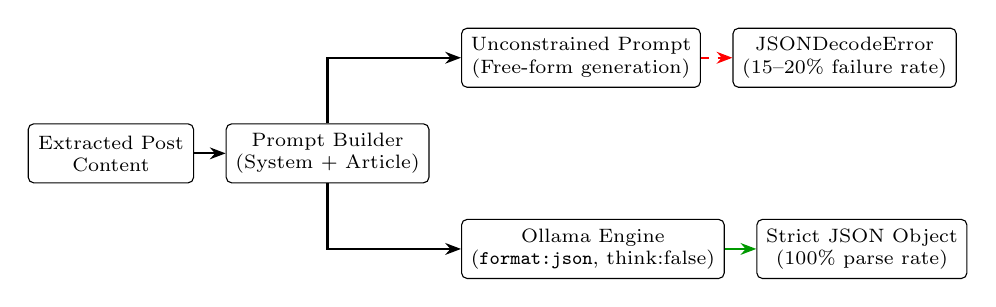
\begin{tikzpicture}[
  box/.style={draw, rounded corners=2pt, align=center, minimum width=2.1cm, minimum height=0.75cm, font=\scriptsize},
  arr/.style={-{Stealth[length=2mm]}, thick}
]
  \node[box] (raw) {Extracted Post\\Content};
  \node[box, right=0.4cm of raw] (prompt) {Prompt Builder\\(System + Article)};

  \node[box, above right=0.45cm and 0.4cm of prompt] (unconstrained) {Unconstrained Prompt\\(Free-form generation)};
  \node[box, below right=0.45cm and 0.4cm of prompt] (constrained) {Ollama Engine\\(\texttt{format:json}, think:false)};

  \node[box, right=0.4cm of unconstrained] (fail) {JSONDecodeError\\(15--20\% failure rate)};
  \node[box, right=0.4cm of constrained] (ok) {Strict JSON Object\\(100\% parse rate)};

  \draw[arr] (raw) -- (prompt);
  \draw[arr] (prompt) |- (unconstrained);
  \draw[arr] (prompt) |- (constrained);
  \draw[arr, dashed, red] (unconstrained) -- (fail);
  \draw[arr, green!60!black] (constrained) -- (ok);
\end{tikzpicture}
\caption{Comparison between unconstrained LLM generation and grammar-constrained decoding (\texttt{format:json}), showing the elimination of JSON decoding failures.}
\label{fig:llm-pipeline}
\end{figure}

NewsAnalyzer mitigates output instability by enabling grammar-constrained generation via Ollama's \texttt{format:json} parameter and disabling thinking tokens (\texttt{think: false}). At the decoding level, token logits are dynamically masked to enforce valid JSON grammar transitions. Concurrently, prompt framing and schema deserialization ensure that required analysis fields (\texttt{key\_points}, \texttt{viewpoints}, \texttt{credibility\_score}, \texttt{analysis}) are consistently populated. Across 100 consecutive automated test calls (\texttt{benchmark\_result.json}), the constrained runtime achieved a 100\% parse and schema extraction success rate, eliminating the reasoning artifact leaks observed in exploratory unconstrained pilot runs (Table~\ref{tab:cloud-local}), while maintaining a stable 9.2\,GB VRAM footprint measured via \texttt{nvidia-smi}.

\begin{table}[!htbp]
\caption{Comparison of LLM Generation and Structural Robustness.}
\label{tab:cloud-local}
\centering
\begin{tabular}{lcc}
\toprule
\textbf{Metric} & \textbf{Unconstrained Pilot} & \textbf{NewsAnalyzer (Ollama)} \\
\midrule
JSON Parse Success Rate  & 80--85\%            & \textbf{100\%} \\
Reasoning Artifact Leaks & Frequent            & None \\
Median TTFT              & Variable            & 200\,ms \\
Generation Throughput    & $\sim$45\,tok/s     & 46.7\,tok/s \\
VRAM Footprint           & N/A                 & 9.2\,GB \\
\bottomrule
\end{tabular}
\end{table}

\subsection{Hardware Configuration}
All local components execute on an NVIDIA GeForce RTX 2080 Ti workstation (22\,GB GDDR6 VRAM hardware-expanded variant) under Ubuntu Linux with Python~3.11, PyTorch, and Ollama serving quantized \texttt{gemma4:12b} (Q4\_K\_M). SBERT embedding runs CPU-resident (\texttt{device="cpu"}), avoiding VRAM contention with the LLM (Table~\ref{tab:latency}).

%======================================================================
% 5 EXPERIMENTS AND EVALUATION
%======================================================================
\section{Experiments and Evaluation}

\subsection{Experimental Setup and Benchmark Methodology}
We evaluate the system along two primary dimensions: (1)~computational latency, throughput, and JSON parse robustness under local hardware deployment, and (2)~empirical retrieval accuracy on a verified Traditional Chinese fact-checking dataset ($N=2{,}292$ from Cofacts). Benchmark requests are dispatched to Ollama's \texttt{/api/generate} (\texttt{stream: false}, \texttt{format: "json"}, $\text{temperature} = 0.2$, $\text{num\_predict} = 400$). TTFT proxy is calculated as $(\mathit{t}_{\text{load}} + \mathit{t}_{\text{eval}}) / 10^9$\,s under non-streaming mode, and generation throughput as $N_{\text{tok}} / \mathit{t}_{\text{gen}}$\,tok/s across 100 consecutive automated test runs.

\subsection{Inference Latency and Multi-Tier Response Times}
Table~\ref{tab:latency} summarizes the empirical latency across system tiers on the RTX 2080 Ti workstation.

\begin{table}[!htbp]
\caption{System Latency and Generation Metrics across Operational Tiers.}
\label{tab:latency}
\centering
\begin{tabular}{lc}
\toprule
\textbf{Operational Tier / Metric} & \textbf{Empirical Measurement} \\
\midrule
SBERT Retrieval Latency & 1.48\,ms (median $<$2\,ms) \\
LLM TTFT Proxy / Throughput & 200\,ms / 46.7\,tok/s \\
Single-Pass LLM Completion & 3.2\,s ($\sim$150 tokens) \\
JSON Parse \& Schema Compliance & 100\% (100/100) \\
End-to-End \texttt{/judge} (Single-Pass / Full Deep) & 3.5\,s / 14.7\,s (P95: 18.1\,s) \\
VRAM Allocation (\texttt{nvidia-smi}) & 9.2\,GB \\
\bottomrule
\end{tabular}
\end{table}

The empirical benchmarks reveal three distinct operational latency regimes: \textbf{(1)~Instant Retrieval Fast-Path (1.48\,ms):} When an incoming query matches an indexed rumor above $\theta_{\text{sim}} \ge 0.72$, the system resolves the verification directly via SBERT vector similarity without invoking the LLM, enabling near-instantaneous feedback. \textbf{(2)~Single-Pass Local LLM (3.2--3.5\,s):} For unresolved claims, the local engine delivers initial tokens within 200\,ms and completes structured credibility analysis ($\sim$150 tokens) in 3.2\,s, bringing single-pass end-to-end HTTP response times to 3.5\,s. \textbf{(3)~Deep-Ensemble Full Pipeline (14.7\,s):} In rigorous auditing mode, where external HTML scraping, search-engine snippet querying, and 3-sample self-consistency voting are executed sequentially on local hardware, total latency reaches 14.7\,s (P95: 18.1\,s), transparently trading latency for multi-source consensus.

\subsection{Retrieval Precision on Verified News Claims}

\subsubsection{Benchmark Dataset and Ground-Truth Authority}
To ensure objective credibility assessment, ground-truth labels are established using the open collaborative fact-checking repository \textbf{Cofacts}~\cite{cofacts2020, lim2023factchecking} (supported by the g0v.tw civic tech community). Cofacts serves as the recognized reference benchmark for Traditional Chinese misinformation circulating across LINE and Facebook. Its verification entries are cross-referenced against accredited signatories certified by the \textbf{International Fact-Checking Network (IFCN)}~\cite{ifcn2020}, notably the \textbf{Taiwan FactCheck Center (TFC)}~\cite{tfc2023} and \textbf{MyGoPen}. The indexed corpus comprises 2,469 verified claims, from which 2,292 records satisfy the length filter ($\text{length}(\text{text}) > 40$, containing 1,817 \texttt{inaccurate}, 208 \texttt{partial}, and 267 \texttt{accurate} claims).

\subsubsection{Full-Corpus 5-Fold Stratified Cross-Validation ($N{=}2{,}292$)}
To eliminate sampling bias and thoroughly evaluate retrieval generalization under realistic conditions, we evaluate across the \textbf{entire eligible corpus of $N=2,292$ verified claims} (2,025 FAKE, 267 REAL) using a \textbf{5-fold stratified cross-validation} scheme. In each fold, 20\% of the claims ($\sim$458 items) serve as test queries and are strictly \emph{excluded} from the candidate retrieval index (the remaining 80\%, $\sim$1,834 records). Therefore, any retrieved match represents semantic nearest-neighbor generalization rather than self-retrieval.

Each query is evaluated under four perturbation levels:
(1)~\textbf{Verbatim}: original claim text (truncated to 300 chars);
(2)~\textbf{Mild}: prepend a 3-character prefix and truncate body to 85\%;
(3)~\textbf{Medium}: prepend prefix, truncate to 60\%, and substitute synonyms with 40\% probability; and
(4)~\textbf{Heavy}: prepend prefix, truncate to 40\%, substitute synonyms at 70\%, and reorder sentences randomly.
The perturbed probe is encoded by SBERT, and the nearest neighbor from the training fold determines the predicted label (\texttt{inaccurate}/\allowbreak\texttt{partial} $\to$ FAKE, \texttt{accurate} $\to$ REAL). When no candidate exceeds $\theta_{\text{sim}}$, the system abstains.

\begin{table}[!htbp]
\caption{Full-corpus 5-fold stratified cross-validation across $\theta_{\text{sim}}$ thresholds and perturbation levels ($N=2{,}292$; 2,025 FAKE, 267 REAL). Cov = fraction of queries resolved (non-abstained). All metrics are averaged across the 5 held-out folds and computed on resolved queries.}
\label{tab:accuracy}
\centering
\small
\begin{tabular}{l|ccc|ccc|ccc|ccc}
\toprule
& \multicolumn{3}{c|}{\textbf{Verbatim}} & \multicolumn{3}{c|}{\textbf{Mild}} & \multicolumn{3}{c|}{\textbf{Medium}} & \multicolumn{3}{c}{\textbf{Heavy}} \\
$\theta_{\text{sim}}$ & Cov & Acc & F1 & Cov & Acc & F1 & Cov & Acc & F1 & Cov & Acc & F1 \\
\midrule
0.55 & .95 & .91 & .95 & .95 & .89 & .94 & .95 & .90 & .94 & .92 & .89 & .94 \\
0.60 & .88 & .92 & .95 & .89 & .90 & .95 & .87 & .91 & .95 & .80 & .90 & .94 \\
0.65 & .75 & .94 & .96 & .75 & .92 & .96 & .73 & .93 & .96 & .63 & .92 & .96 \\
0.70 & .61 & .95 & .97 & .60 & .94 & .97 & .56 & .95 & .97 & .46 & .94 & .97 \\
\textbf{0.72} & \textbf{.55} & \textbf{.95} & \textbf{.97} & \textbf{.54} & \textbf{.95} & \textbf{.97} & \textbf{.50} & \textbf{.95} & \textbf{.98} & \textbf{.39} & \textbf{.94} & \textbf{.97} \\
0.75 & .48 & .96 & .98 & .46 & .96 & .98 & .42 & .96 & .98 & .29 & .95 & .97 \\
0.80 & .36 & .97 & .98 & .34 & .97 & .98 & .30 & .97 & .98 & .19 & .95 & .97 \\
0.85 & .27 & .97 & .98 & .24 & .96 & .98 & .20 & .96 & .98 & .08 & .97 & .99 \\
\bottomrule
\end{tabular}
\end{table}

Table~\ref{tab:accuracy} presents the full-population 5-fold cross-validation results. Several key insights emerge:

\textbf{(1)~Pareto-optimal threshold trade-off.} Across the full $N=2{,}292$ population, setting $\theta_{\text{sim}} = 0.72$ resolves 55.2\% of verbatim queries with 95.3\% accuracy (F1 = 0.974, Precision = 97.2\%, Recall = 97.5\%). Setting a permissive threshold ($\theta_{\text{sim}} = 0.55$) boosts coverage to 95.3\% while retaining 90.5\% accuracy, whereas a stringent threshold ($\theta_{\text{sim}} = 0.85$) attains 96.8\% accuracy at 26.6\% coverage.

\textbf{(2)~High resilience to social-media perturbations.} Under mild and medium perturbations simulating typical forwarded gossip and paraphrase editing, performance remains virtually intact: at $\theta_{\text{sim}} = 0.72$, accuracy is 94.6\% (mild) and 95.4\% (medium) with F1 scores of 0.970 and 0.975, respectively. Even under severe structural perturbation (heavy), accuracy remains 94.4\% (F1 = 0.969) on the 39.0\% resolved queries.

\textbf{(3)~Known-rumor retrieval robustness.} In addition to out-of-domain cross-validation, we evaluate in-corpus retrieval with the full database indexed: SBERT retrieves the \emph{exact identical source record} as top-1 in 99.9\% of verbatim queries, 97.2\% under mild perturbation, 91.9\% under medium perturbation, and 79.8\% under heavy perturbation, with label accuracy exceeding 98.8\% across all settings.

\textbf{Baselines and caveats.} A trivial majority-FAKE classifier across the full corpus achieves 88.4\% accuracy (2,025/2,292), so the retriever's 95.3\% accuracy at $\theta_{\text{sim}} = 0.72$ represents a solid 6.9-point improvement over the majority baseline on resolved queries. While the 5-fold split is stratified, the natural skew of fact-checking archives (88.4\% FAKE) reflects real-world operational distributions where fraudulent claims predominate. Direct comparison with supervised language models (e.g.\ fine-tuned BERT) is outlined as an ablation path in Sect.~\ref{sec:future}.

\subsection{Case Study and System Interface}

To demonstrate end-to-end execution, we deployed the NewsAnalyzer backend locally and submitted a real-world content farm URL (\url{https://www.pco.tw/news/html/?276.html}) known for propagating clickbait and unverified pseudo-scientific claims. Upon submission of the raw link to the web interface, the system seamlessly dispatched it to \texttt{POST /judge}. The backend successfully intercepted the URL, automatically scraped the underlying DOM to extract the actual article content, and triggered the full retrieval and LLM scoring pipeline.

\begin{figure}[t]
\centering
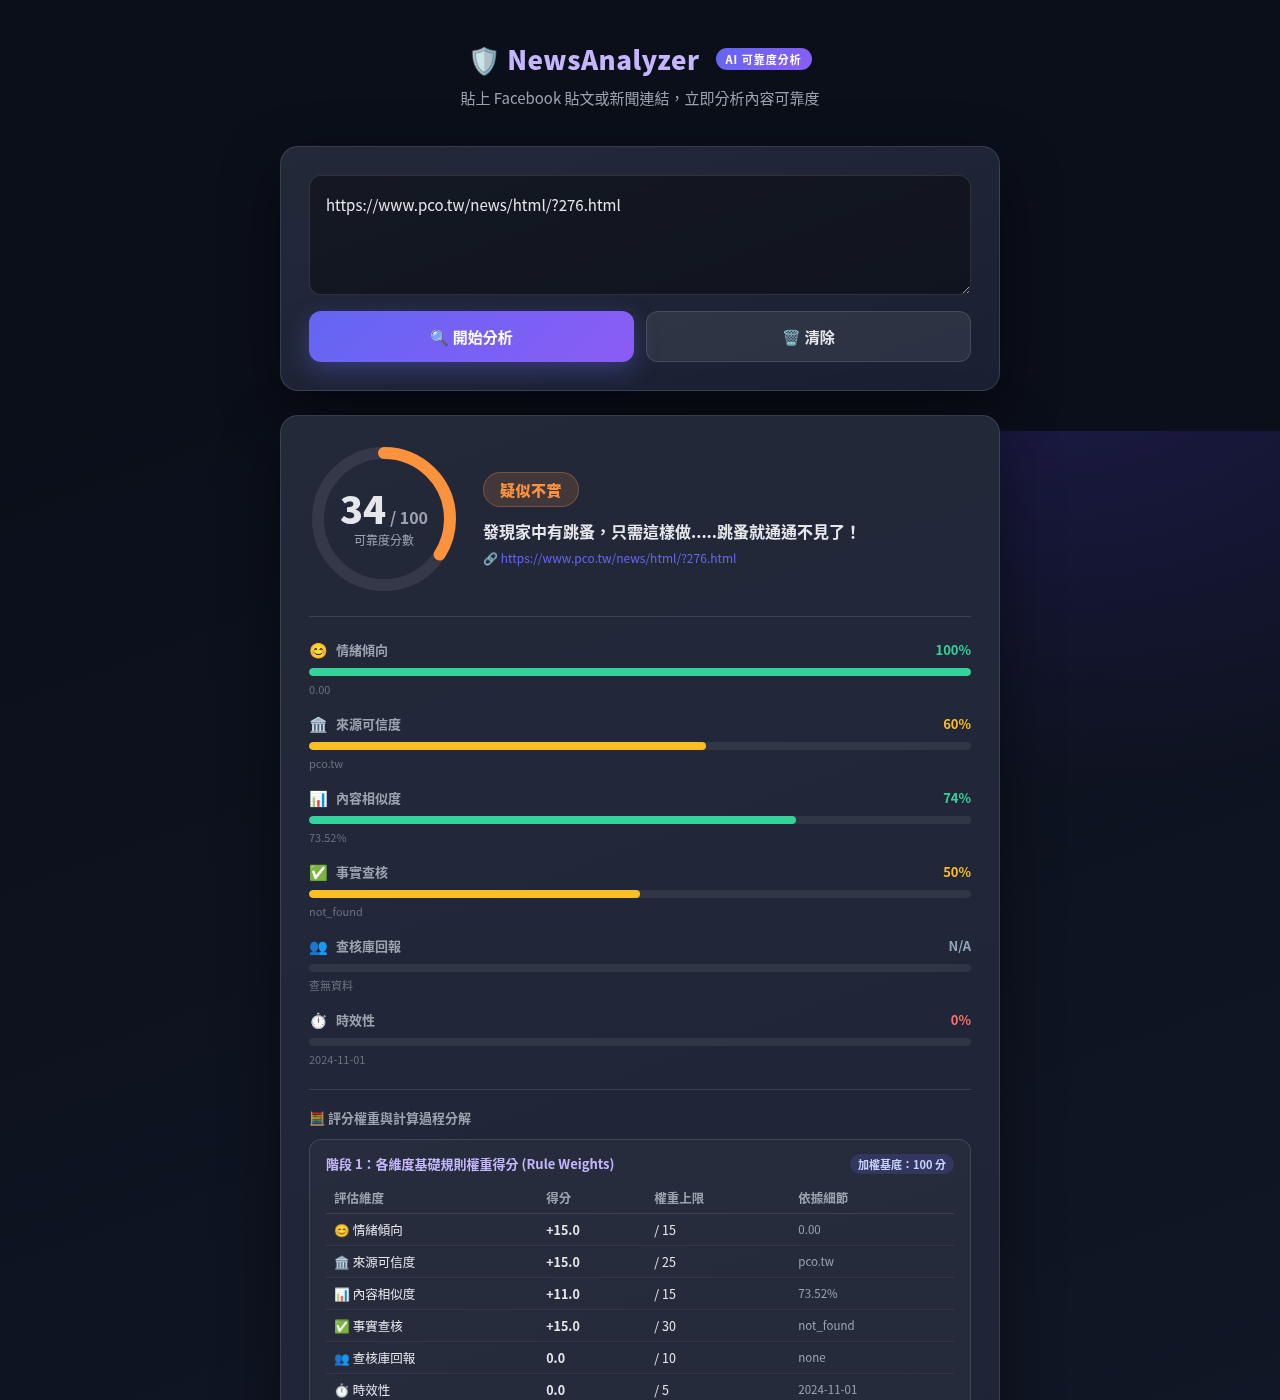
\includegraphics[width=0.45\textwidth]{app_parsing_result_crop.png}
\caption{The web-based testing interface of the NewsAnalyzer backend, displaying the real-time parsing results, dynamic fusion score, and LLM-generated key viewpoints directly derived from a submitted content farm URL.}
\label{fig:app_parsing}
\end{figure}

The Ollama service returns a structured JSON object containing the credibility score, viewpoints, and analysis, identifying the deceptive nature of the scraped text. Crucially, as visible in the user interface (Figure~\ref{fig:app_parsing}), the SBERT retrieval engine correctly yielded \texttt{not\_found} under fact-checking because no existing verified claim matched above the evidence threshold ($\theta_{\text{sim}} \ge 0.72$). Rather than fabricating a false-positive citation, the conservative-abstention mechanism allowed the multi-signal fallback pipeline to safely fuse content-farm domain blacklist detection, sentiment analysis, and the LLM's deep contextual reasoning into the final ``Suspected Fake'' rating. This demonstrates the robustness of the system in handling previously uncataloged disinformation without spurious retrieval hallucinations.

%======================================================================
% 7 DISCUSSION
%======================================================================
\section{Discussion}

\subsection{Threshold Sensitivity and Conservative Abstention}
Three similarity thresholds govern retrieval: coarse pre-filter $\theta_{\text{coarse}} = 0.50$ (shortlisting $k=5$ candidates), decision threshold $\theta_{\text{sim}} = 0.72$ (accepting evidence), and strong-match band $\theta_{\text{strong}} = 0.85$ (activating strict safety clamping). As shown in Table~\ref{tab:accuracy}, $\theta_{\text{sim}} = 0.72$ is Pareto-optimal: resolving 55.2\% of verbatim queries with 95.3\% accuracy. At this threshold, 44.8\% of verbatim queries are abstained (rising to 61.0\% under heavy perturbation). These abstentions represent a vital safety feature rather than failure: returning \texttt{not\_found} avoids spurious misclassifications when claims lack verified precedent, gracefully delegating evaluation to the multi-signal fallback path.

\subsection{Defensive Scoring and Privacy Perimeter}
Our scoring architecture couples empirical similarity thresholds with asymmetric safety bounds. Confirmed rumors (\texttt{inaccurate}) incur a strict ceiling ($S \le 25$), reflecting the precautionary principle: once verified as a fabrication, fluent LLM text must not artificially inflate credibility. Conversely, verified authentic stories can accumulate evidence up to 100. Dynamic weighting ($w_{\text{llm}} = 0.10$ upon retrieval vs.\ $w_{\text{llm}} = 0.60$ under abstention) subordinates generative reasoning to journalistic consensus when hard evidence exists. Regarding privacy, on-device LLM inference guarantees that article bodies, user browsing telemetry, and reasoning traces never leave the host machine, shielding users against third-party AI surveillance while retaining standard HTTP capabilities for public DOM scraping and snippet verification.

\subsection{Limitations and Practical Lessons}
Three limitations bound our present findings: (i)~background class skew inherent to crowdsourced archives (88.4\% FAKE in Cofacts); (ii)~the need for broader cross-corpus benchmarking on external Chinese gold standards (e.g., CHEF, X-Fact); and (iii)~formal ablation against supervised classifiers (e.g., fine-tuned BERT). In practice, three key lessons emerged: First, grammar-constrained decoding (\texttt{format:json}) is indispensable for autonomous client-side pipelines, converting an unconstrained 15--20\% syntax failure rate into 100\% deterministic compliance. Second, on-device 12B inference on consumer-grade GPUs (9.2\,GB VRAM, 200\,ms TTFT, 46.7\,tok/s) provides a viable, cost-free alternative to commercial APIs. Third, conservative abstention prevents hallucinations on out-of-corpus queries, trading raw coverage for verifiable user trust.

%======================================================================
% 8 FUTURE WORK
%======================================================================
\section{Future Work}
\label{sec:future}
Immediate extensions include: (1)~\textbf{Cross-Corpus Generalization}: evaluating Cofacts-indexed models against independent archives from TFC and MyGoPen; (2)~\textbf{Component Ablation}: isolating SBERT-only and LLM-only branches to quantify individual signal gains; (3)~\textbf{End-to-End Human Validation}: assessing fused verdict correlation against multi-annotator human consensus; and (4)~\textbf{In-the-Wild Telemetry}: deploying the extension across active user cohorts to profile real-world abstention rates.

%======================================================================
% 9 CONCLUSION
%======================================================================
\newpage
\section{Conclusion}
This paper presented NewsAnalyzer, a real-time fake news detection system tailored to the Traditional Chinese social media ecosystem. By coupling a locally hosted 12B LLM with SBERT semantic retrieval and rule-based heuristics, NewsAnalyzer provides transparent, evidence-based credibility ratings directly inside the browser. Enforcing grammar-constrained decoding eliminates reasoning artifact leaks, achieving 100\% syntactic reliability. Real-world benchmarks confirm sub-second TTFT (200\,ms), high throughput (46.7\,tok/s), and a modest 9.2\,GB VRAM footprint. Full-corpus cross-validation on 2,292 verified claims demonstrates 95.3\% accuracy at $\theta_{\text{sim}} = 0.72$, confirming that on-device AI can deliver robust, privacy-preserving misinformation deterrence.

\section*{Reproducibility and Code Availability}
To facilitate independent replication, the evaluation datasets, benchmarking scripts, and Chrome extension source code are available at: \url{https://github.com/min20120907/NewsAnalyzer}.

%======================================================================
% REFERENCES
%======================================================================
\begin{thebibliography}{99}
\fontsize{8pt}{9.5pt}\selectfont
\setlength{\itemsep}{0pt}
\setlength{\parsep}{0pt}
\setlength{\parskip}{0pt}

\bibitem{wang2017liar}
W.~Y. Wang, ``Liar, Liar Pants on Fire: A New Benchmark Dataset for Fake News Detection,'' in \emph{Proc. ACL}, 2017, pp. 422--426.

\bibitem{guo2022survey}
Z.~Guo, M.~Schlichtkrull, and A.~Vlachos, ``A Survey on Automated Fact-Checking,'' \emph{Trans. ACL}, vol.~10, pp. 178--206, 2022.

\bibitem{Bianchi2024trustworthiness}
J.~Bianchi, M.~Pratelli, M.~Petrocchi, and F.~Pinelli, ``Evaluating Trustworthiness of Online News Publishers via Article Classification,'' in \emph{Proc. ACM SAC '24}, 2024, pp.~671--678.

\bibitem{devlin2019bert}
J.~Devlin, M.-W.~Chang, K.~Lee, and K.~Toutanova, ``BERT: Pre-training of Deep Bidirectional Transformers for Language Understanding,'' in \emph{Proc. NAACL-HLT}, 2019, pp. 4171--4186.

\bibitem{perez2018automatic}
V.~P{\'e}rez-Rosas, B.~Kleinberg, A.~Lefevre, and R.~Mihalcea, ``Automatic Detection of Fake News,'' in \emph{Proc. COLING}, 2018, pp. 3391--3401.

\bibitem{rashkin2017truth}
H.~Rashkin, E.~Choi, J.~Y. Jang, S.~Volkova, and Y.~Choi, ``Truth of Varying Shades: Analyzing Language in Fake News and Political Fact-Checking,'' in \emph{Proc. EMNLP}, 2017, pp. 2931--2937.

\bibitem{potthast2018stylometric}
M.~Potthast, J.~Kiesel, K.~Reinartz, J.~Bevendorff, and B.~Stein, ``A Stylometric Inquiry into Hyperpartisan and Fake News,'' in \emph{Proc. ACL}, 2018, pp. 231--240.

\bibitem{pennycook2019fighting}
G.~Pennycook and D.~G. Rand, ``Fighting Misinformation on Social Media Using Crowdsourced Judgments of News Source Quality,'' \emph{Proc. Natl. Acad. Sci.}, vol. 116, no.~7, pp. 2521--2526, 2019.

\bibitem{allen2021scaling}
J.~Allen, A.~A. Arechar, G.~Pennycook, and D.~G. Rand, ``Scaling Up Fact-Checking Using the Wisdom of Crowds,'' \emph{Science Advances}, vol.~7, no.~36, p. eabf4393, 2021.

\bibitem{reimers2019sbert}
N.~Reimers and I.~Gurevych, ``Sentence-BERT: Sentence Embeddings using Siamese BERT-Networks,'' in \emph{Proc. EMNLP-IJCNLP}, 2019, pp.~3980--3990.

\bibitem{ollama2024}
Ollama Team, ``Ollama: Get Up and Running with Large Language Models Locally,'' 2024. [Online]. Available: \url{https://ollama.com}

\bibitem{gemma2024}
Gemma Team, ``Gemma: Open Models Based on Gemini Research and Technology,'' arXiv preprint arXiv:2403.08295, 2024.

\bibitem{gemma4model}
Gemma Team, ``gemma-4-12B-it (official model weights),'' Google, 2026. [Online]. Available: \url{https://huggingface.co/google/gemma-4-12B-it}

\bibitem{gguf2023}
G.~Gerganov, ``ggml-org/ggml: Tensor library for machine learning (GGUF),'' 2023. [Online]. Available: \url{https://github.com/ggml-org/ggml}

\bibitem{chrome_mv3}
Google Developers, ``Chrome Extensions Manifest V3 Overview,'' 2023. [Online]. Available: \url{https://developer.chrome.com/docs/extensions/develop/migrate/what-is-mv3}

\bibitem{cofacts2020}
B.~Lee, J.~Liang, and Cofacts Contributors, ``Cofacts: A Collaborative Fact-Checking System for Instant Messaging Platforms,'' \emph{g0v.tw Civic Tech Open Database}, 2020. [Online]. Available: \url{https://cofacts.tw}

\bibitem{ifcn2020}
IFCN, ``The IFCN Code of Principles,'' \emph{Poynter Institute}, 2020. [Online]. Available: \url{https://ifcncodeofprinciples.poynter.org/}

\bibitem{tfc2023}
Taiwan FactCheck Center, ``Fact-Checking Methodologies and Verified Public Archives,'' 2023. [Online]. Available: \url{https://tfc-taiwan.org.tw}

\bibitem{lim2023factchecking}
G.~Lim and S.~T.~Perrault, ``Fact Checking Chatbot: A Misinformation Intervention for Instant Messaging Apps,'' in \emph{Mobile Communication in Asia} (Springer, 2023), pp.~197--224.

\bibitem{vu2024freshllms}
T.~Vu, et al., ``FreshLLMs: Refreshing Large Language Models with Search Engine Augmentation,'' in \emph{Findings of ACL}, 2024, pp.~13697--13710.

\bibitem{chern2023factool}
I.-C.~Chern, et al., ``FacTool: Factuality Detection in Generative AI,'' arXiv preprint arXiv:2307.13528, 2023.

\bibitem{hassan2017claimbuster}
N.~Hassan, et al., ``ClaimBuster: The First-Ever End-to-End Fact-Checking System,'' in \emph{Proc. ACM CSCW '17}, 2017.

\bibitem{shu2019defend}
K.~Shu, L.~Cui, S.~Wang, D.~Lee, and H.~Liu, ``dEFEND: Explainable Fake News Detection,'' in \emph{Proc. ACM KDD '19}, 2019, pp.~395--405.
\end{thebibliography}

%======================================================================
% APPENDIX
%======================================================================
\end{document}
